%!TEX root = main.tex

	\section{Study Results}
	\bchange{
	 We introduce the study findings for each task starting from the narrowest scope of \emph{individual} visualizations to the widest scope of \emph{overall} dataset understanding.
}
\change{\stitle{RQ1: How are \emph{individual} selected visualizations in the dashboard perceived subjectively by the users?}
}
\npar Using click-stream data logged from the user study, 
we recorded whether a
participant \bchange{labeled each} visualization 
in the dashboard as interesting, not interesting, 
or left the visualization unselected. 
Table~\ref{table:interestingScore} summarizes 
\bchange{the} counts of visualizations 
marked as interesting or not interesting 
aggregated across conditions. 
We also normalize the interestingness count 
by the total number of selected visualizations 
to account for variations in how some participants 
select more visualizations than others. 
The results indicate that participants who 
used \system\ \change{saw} more 
visualizations that they found interesting compared 
to the \BFS and \cluster \change{\xspace conditions}. 
\change{While  \bchange{this task is 
inherently subjective, with many possible
reasons why a participant may have marked a visualization 
as interesting, this result is indicative of the fact that the
selected visualizations were deemed to be relevant
by users. We will drill into possible reasons why in the next section.}}
\begin{table}[h!]
\vspace{-5pt}
	\centering
	\begin{tabular}{lrrr}
	 \small{Condition}             &   \small{\system} &   \small{\BFS} &   \small{\cluster} \\
	\hline
	 \small{Interesting}            &  \cellcolor{blue!25}       66    & 61    &      51   \\
	 \small{Not Interesting}        &  \cellcolor{blue!25}       10    & 20    &      22   \\
	 \small{Interesting (Normalized)} &   \cellcolor{blue!25}       0.87 &  0.75 &       0.7 \\
	\end{tabular}
	\caption{Total counts of visualizations marked as interesting or not interesting across the different conditions. \system leads to more visualizations marked as interesting and fewer visualizations marked as uninteresting.}
	\label{table:interestingScore}
	\vspace{-20pt}
\end{table}
\stitle{\change{RQ2: How well do dashboard visualizations provide users with an accurate \bchange{understanding} of \emph{related} visualizations?}}
\npar 
\bchange{As discussed in Section~\ref{sec:problem}, 
contextualizing visualizations correctly with informative
references can help prevent users from falling prey to 
drill-down fallacies. To this end,
the prediction task aims to assess whether
users can employ visualizations in the dashboard
to correctly predict unseen ones. 
Indeed, if the dashboard is constructed well,
one would expect that only the visualizations
that are not very surprising relative to their informative parents
would be excluded from the dashboard 
(i.e., their deviation from their informative parents is not large).} 
\begin{figure}[h!]
\centering
\vspace{-15pt}
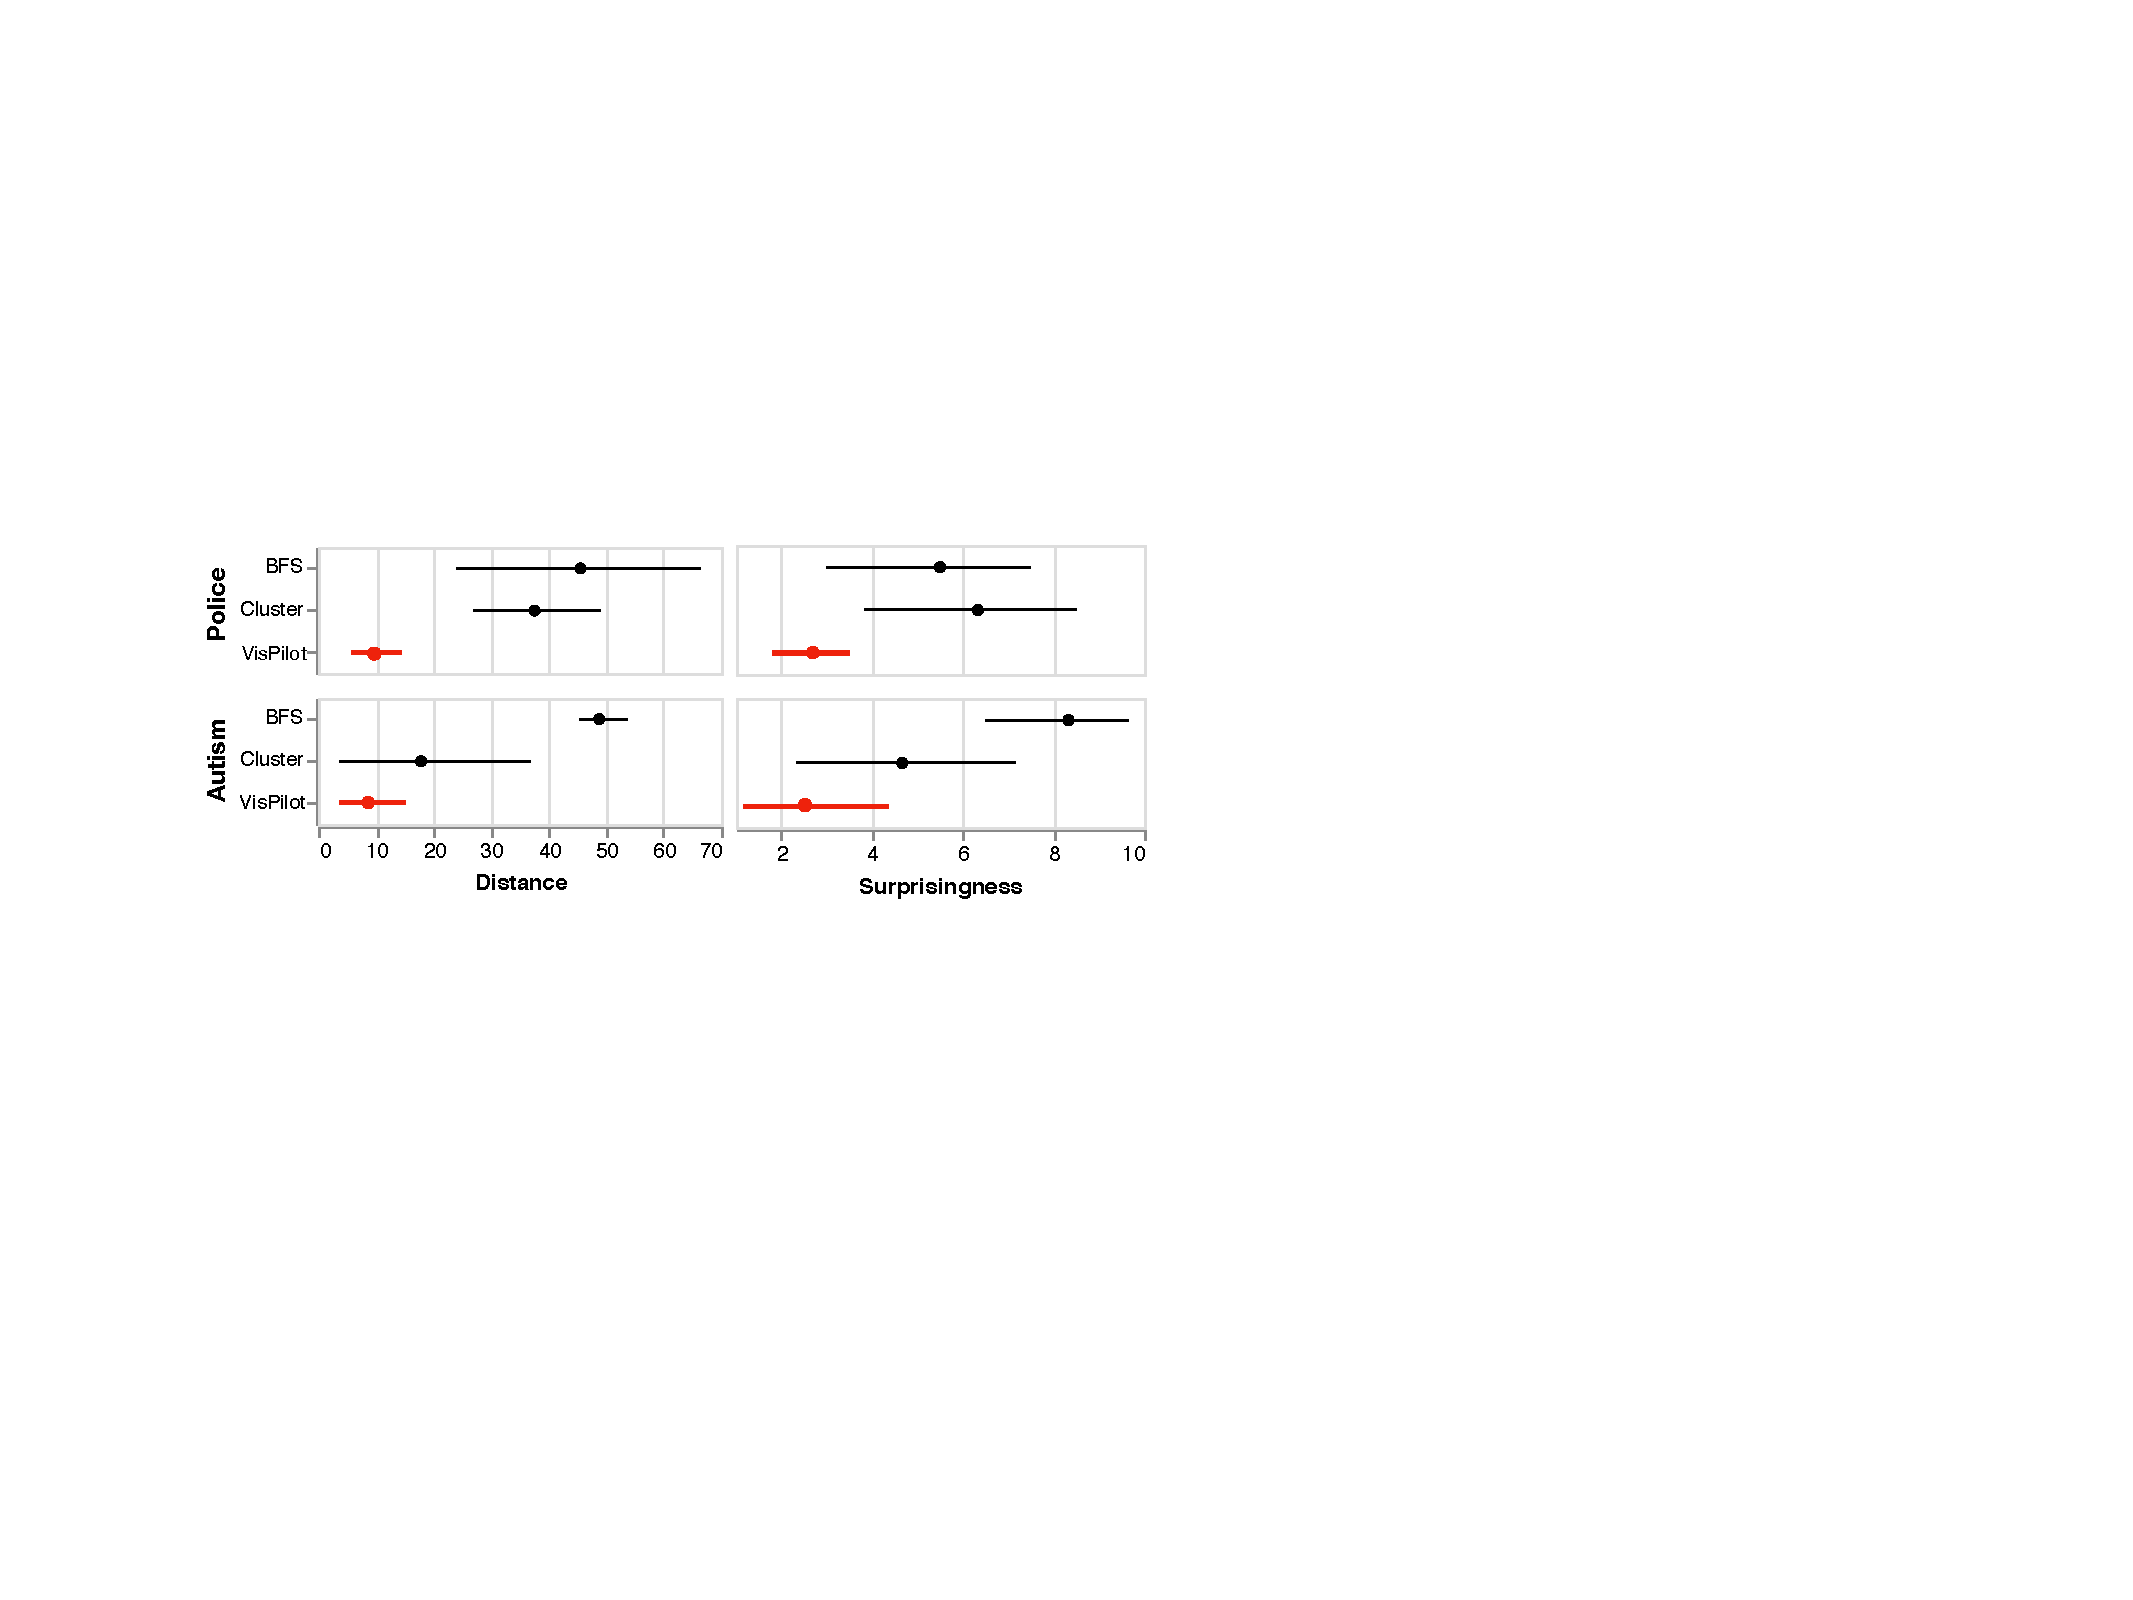
\includegraphics[width=0.95\linewidth]{figures/prediction_surprisingness_distance.pdf}
\caption{Left: Euclidean distance between predicted and ground truth. In general, predictions made using \system are closer to ground truth. Right: Surprisingness rating reported by users after seeing the actual visualizations on a Likert scale of 10. \system participants had a more accurate mental model of the unseen visualization and therefore reported less surprise than compared to the baselines.}
\vspace{-10pt}
\label{fig:distance}
\end{figure}
\par The accuracy of participants' predictions 
\bchange{is measured using}
the Euclidean distance between \change{their} predicted distributions and ground truth data distributions. 
As shown in Figure~\ref{fig:distance} (left), 
predictions made using \system\ (highlighted in red) 
were closer to the actual distribution than compared to the baselines, 
as indicated by the smaller Euclidean distances. 
Figure~\ref{fig:distance} (right) also shows 
that \system participants \change{were able to more 
accurately reason about the expected properties of 
unseen data subsets \bchange{(or visualizations)}, 
since they rated the resulting visualizations to be less surprising}. 
\cluster may have performed better \bchange{for} 
the Police dataset than it did \bchange{for} 
the Autism \bchange{one},
\bchange{for the same reason as in the attribute ranking task,
where more univariate visualizations happened to be selected,
described subsequently.} 


\par We also compute the variance of participants' predictions across the same condition. In this case, low variance implies 
that 
\bchange{there is consistency or agreement
between the predictions of participants 
who consumed the same
dashboard}, 
whereas high variance implies that the 
dashboard did not convey a clear data-driven story 
that could guide participants' predictions. 
So instead, participants \bchange{had to rely on prior knowledge or} guessing to 
\bchange{inform} their prediction(s). These trends can be observed in both Figure~\ref{fig:distance} and in more detail in Figure \ref{fig:actual_predictions}, where the prediction variance amongst participants who used \system\ is generally lower than the variance for the baselines. 
\bchange{Overall, \system provides participants 
with a more accurate and consistent model of 
\emph{related} visualizations.}
\begin{figure}[h!]
\vspace{-10pt}
\centering
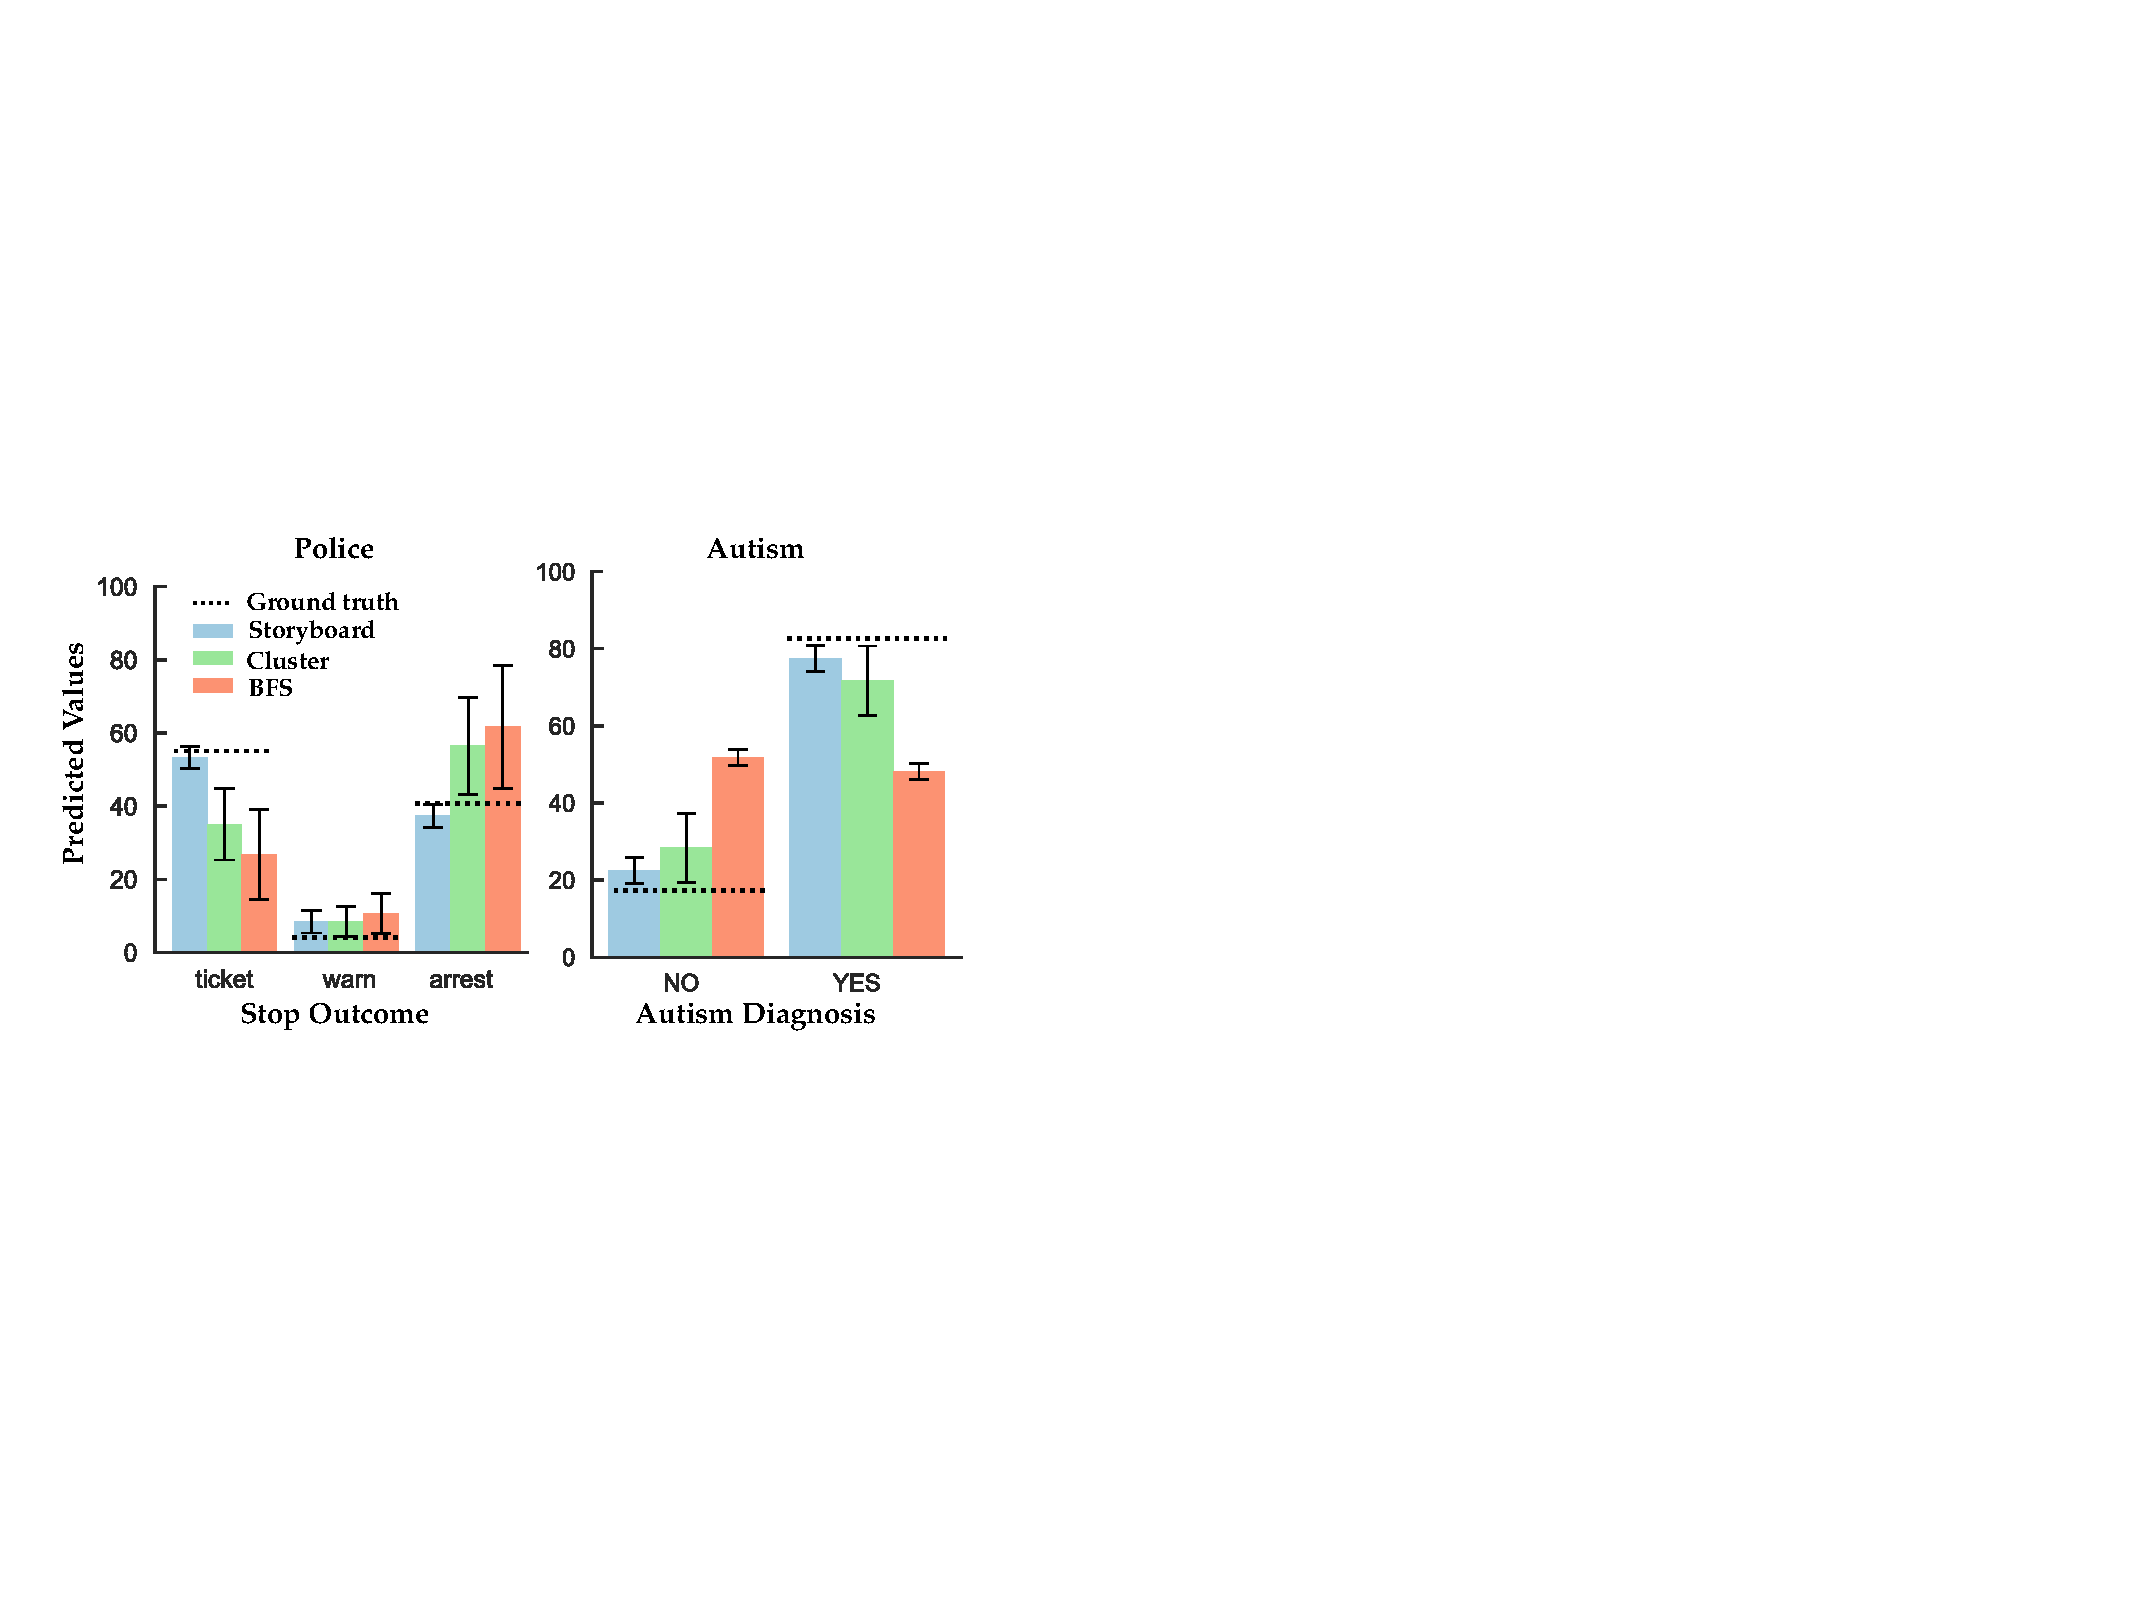
\includegraphics[width=0.85\linewidth]{figures/prediction.pdf}
\vspace{-10pt}
\caption{Mean and variance of predicted values. Predictions based on \system exhibit lower variance \change{(error bars)} and closer proximity to the ground truth values (dotted).\agp{Fix}}
\label{fig:actual_predictions}
\vspace{-10pt}
\end{figure}
\change{
	\stitle{RQ3: How well does the dashboard convey information regarding \bchange{the} \emph{overall} dataset schema?}% information regarding the relative importance of different attributes
\npar 
\bchange{We use the common  task 
of judging the relative importance of attributes 
as an indicator of the participants' overall understanding.}}
To determine \bchange{ground truth} attribute importance, 
we computed the Cramer's V statistics 
between attributes to be ranked 
and the attributes of interest. 
Cramer's V is \bchange{commonly used for} 
determining 
the strength of association between categorical attributes~\cite{McHugh2013}. We deem an attribute as important if it has one 
of the top-three\footnote{\change{This relevancy cutoff is visually-determined via the elbow method to indicate which rank the Cramer's V score drops off significantly.}} Cramer's V scores amongst all attributes of the dataset. 
For the list of rankings provided by each participant, 
we first remove attributes \bchange{that} participants chose not to rank. 
We compute the F-scores and average precision (AP) at k 
\bchange{relative to the ground truth
for various values of $k$} 
\tr{(from 1 up to the number of ranked attributes, with k values corresponding to attributes ranked as ties deduplicated)\agp{I don't understand this parenthetical note so I have moved it to the TR)}}. 
Table \ref{table:ranking_results} \change{reports the average across participants} in each condition, after picking the best performing $k$ value for each user based on F-score and AP respectively. Both measures capture how accurately participants were able to \bchange{identify} 
the three most important attributes for each dataset.
\begin{table}[ht!]
	\centering
	\vspace{-10pt}
	\begin{tabular}{lllll}
	         & \multicolumn{2}{c}{Police}                                   & \multicolumn{2}{c}{Autism}                                   \\ \hline
	Metric   & F                             & AP                            & F                             & AP                            \\ \hline
	\system  & \cellcolor{blue!25}0.750 & \cellcolor{blue!25}0.867 & 0.723                         & 0.600                         \\ 
	\cluster & 0.739                         & 0.691                         & \cellcolor{blue!25}0.725 & \cellcolor{blue!25}0.665 \\
	\BFS     & 0.739                         & 0.592                         & 0.222                         & 0.200                         \\ 
	\end{tabular}
	\caption{Best AP and F-scores for the attribute ranking task.}
	\label{table:ranking_results}
	\vspace{-20pt}
\end{table}
\par 
\bchange{For this task,
we expected \BFS to have an inherent
advantage, 
since \BFS dashboards consist of all univariate distributions, 
providing more high-level information regarding each attribute.
However,}
both \system and \cluster (which contained more `local' information) 
performed better than \BFS. 
The problem with \BFS is that given 
\bchange{a limited dashboard budget or real-estate of $k = 10$ 
visualizations that could be displayed, 
not all univariate distributions were shown}. 
For the Police dataset, it happened to select several  
important attributes (related to contraband and search) 
to display in the first 10 visualizations. 
However, \bchange{for Autism,} 
only visualizations \bchange{corresponding to} 
binary diagnostic 
questions 1-4 fit in the dashboard. 
So the poor ranking behavior comes from the fact that 
the \BFS generated dashboard failed to display 
the three most important attributes (questions 5, 6 and 9) 
given the limited budget. 
This \bchange{demonstrates \BFS's lack of 
consistency across different datasets,
due to the fact that exhaustive exploration
can only lead to limited understanding of the data.}

\par We see that \system\ performs better 
than \cluster for the Police dataset 
and closely follows \cluster for the Autism dataset. 
It is not entirely surprising that \cluster did well, 
since it is a well-established method for 
summarizing high-dimensional data~\cite{Han2005}. 
For Autism, \cluster happened to pick the majority of visualizations (8/10) as univariate distributions that exhibited high-skew and diversity, 
leading to more informed inference \bchange{of} attribute importance. 
Since clustering seeks visualizations 
that exhibit diversity in the shape of the data distributions, 
it could potentially result in visualizations with many filter combinations. 
For the police dataset, 6 out of 10 visualizations had 
\change{more than 2} filters, 
making it difficult to interpret \change{the visualization} 
without \bchange{an} appropriate context to compare against.

\par \bchange{Overall,} both \BFS and \cluster 
do not provide consistent guarantees for highlighting important visualizations across different datasets. In general, our results indicate that \change{participants} gain a better \bchange{\emph{overall} dataset} understanding regarding attribute importance using \system, with only a few \bchange{targeted visualizations that tell the ``entire story''. This is without \system being explicitly optimized 
for the ranking task}.
